\documentclass[tikz,border=4pt]{standalone}
\usetikzlibrary{arrows.meta,positioning}

\begin{document}
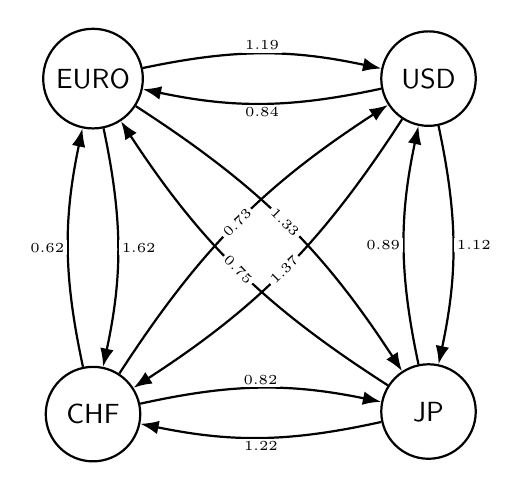
\begin{tikzpicture}[
  >=Latex,
  every node/.style={font=\sffamily},
  circ/.style={draw, thick, circle, minimum size=1.2cm, align=center},
  arrow/.style={->, thick},
  labedge/.style={midway, fill=white, inner sep=1pt, font=\tiny},
  node distance=3cm and 3cm
]
  %--- nodes
  \node[circ]                    (euro) {EURO};
  \node[circ, right=of euro]     (usd)  {USD};
  \node[circ, below=of usd]      (jp)   {JP};
  \node[circ, below=of euro]     (chf)  {CHF};

  %============ ARETES HORIZONTALES ============%
  % EURO <-> USD
  \draw[arrow] (euro) to[bend left=12] node[labedge, above]{1.19} (usd);
  \draw[arrow] (usd)  to[bend left=12] node[labedge, below]{0.84} (euro);

  % CHF <-> JP
  \draw[arrow] (chf)  to[bend left=12] node[labedge, above]{0.82} (jp);
  \draw[arrow] (jp)   to[bend left=12] node[labedge, below]{1.22} (chf);

  %============ ARETES VERTICALES ==============%
  % EURO <-> CHF
  \draw[arrow] (euro) to[bend left=12] node[labedge, right]{1.62} (chf);
  \draw[arrow] (chf)  to[bend left=12] node[labedge, left]{0.62} (euro);

  % USD <-> JP
  \draw[arrow] (usd)  to[bend left=12] node[labedge, right]{1.12} (jp);
  \draw[arrow] (jp)   to[bend left=12] node[labedge, left]{0.89} (usd);

  %============ DIAGONALES =====================%
  % EURO <-> JP
  \draw[arrow] (euro) to[bend left=12] node[labedge, sloped]{1.33} (jp);
  \draw[arrow] (jp)   to[bend left=12] node[labedge, sloped]{0.75} (euro);

  % USD <-> CHF
  \draw[arrow] (usd)  to[bend left=12] node[labedge, sloped]{1.37} (chf);
  \draw[arrow] (chf)  to[bend left=12] node[labedge, sloped]{0.73} (usd);

\end{tikzpicture}
\end{document}
